\documentclass[12pt]{article}
\usepackage[spanish,mexico]{babel}
	\selectlanguage{spanish}
\usepackage{graphicx}
\usepackage{amsmath}
\usepackage{wrapfig}
\usepackage{float}
\usepackage[utf8]{inputenc}

\usepackage{graphicx}
\graphicspath{{images/}}

\usepackage{vmargin}
\setmarginsrb{3 cm}{1 cm}{3 cm}{2.5 cm}{1 cm}{1.5 cm}{1 cm}{1.5 cm}
\usepackage{listings}
\usepackage[usenames,dvipsnames]{color}
	\definecolor{ocre}{RGB}{42,105,21}
	\definecolor{ocre2}{RGB}{47,109,130}
	\definecolor{gray2}{gray}{0.95}
	\lstset{
		language=Python,
		backgroundcolor=\color{gray2},
		basicstyle=\color{black}\small\ttfamily, 
		breakatwhitespace=false,         
		breaklines=true,                 
		captionpos=b,                    
		columns=flexible,
		commentstyle=\color{ocre2}\ttfamily, 
		deletekeywords={...},            
		escapeinside={\%*}{*)},          
		extendedchars=true,             
		frame=single,	                 
		keepspaces=true,                 
		keywordstyle=\color{blue}\bfseries,       
		otherkeywords={*,...},          
		numbers=left,                    
		numbersep=5pt,                   
		numberstyle=\tiny, 
		rulecolor=\color{black},         
		showspaces=false,                
		showstringspaces=false,          
		showtabs=false,                  
		stepnumber=1,                    
		stringstyle=\normalfont\color{ocre},     
		tabsize=2,	                     
		title=\lstname                  
		}

\title{Actividad 5: Movimiento armónico simple:\\ Péndulo}
\author{Martin Alejandro Paredes Sosa}
\date{Marzo, 2016}

\begin{document}
\maketitle
\section{Introducción}
La matemática de un péndulo simple es, en general, compleja. Hacer suposiciones que simplifican la descripción nos permite resolver analíticamente las ecuaciones de movimiento para las oscilaciones de ángulos pequeños.\\
El péndulo simple, es una idealización se un péndulo real, pero en un sistema aislado donde se asume:
\begin{itemize}
	\item La cuerda tiene una masa despreciable, es rígida y se mantiene tensa.
	\item El péndulo se maneja como una masa puntual.
	\item El movimiento es en dos dimensiones trazando un arco.
	\item No pierde energía por fricción o resistencia al aire.
	\item El campo gravitacional es uniforme.
	\item El soporte no se mueve.
\end{itemize}

La ecuación diferencial que representa el movimiento de un péndulo simple es:
\begin{equation}\label{EcDf}
	\frac{d^2\theta}{dt^2} + \frac{g}{\ell}\sin\theta = 0
\end{equation}
donde $g$ es la aceleración de la gravedad, $\ell$ es la longitud del péndulo y $\theta$ es el angulo de desplazamiento \cite{PendWiki}.

%============================================================================================================
\pagebreak
%============================================================================================================

\section{Función \emph{integrate.odeint}}
La ecuación diferencial del péndulo no tiene una solución analítica. Para poder resolverla se utilizan herramientas computacionales. En nuestro caso, para resolverla se utiliza la función \emph{integrate.odeint} de la librería \emph{scipy} de Python \cite{scipy}.

Esta función utiliza los siguientes parámetros:
\begin{itemize}
	\item func: \textit{callable(y, t0, ...)}. Computa la derivada de y en t0.
	\item y0: \textit{arreglo}. Las condiciones iniciales en y. Puede ser un vector.
	\item t:\textit{arreglo}. Secuencia de puntos para los cuales se resolverá y. El valor inicial debe ser el primer valor se la secuencia.
	\item args:\textit{tuple, opcional}. Argumentos extra para la función.
\end{itemize}


%============================================================================================================
\pagebreak

\section{Ejercicio y Resultados}

Esta actividad consistió en realizar un código en python que nos permitiera resolver la ecuación de movimiento de un péndulo simple. Se hizo uso de la librería \emph{scipy.integrate} haciendo uso de la función \textit{odeint}. Para lograr esto se definieron los parámetros de amortiguamiento y de la ecuación \eqref{EcDf}. Se corrieron varias simulaciones variando las condiciones del péndulo.\\

Aquí se tiene el código que se utilizo.

\lstinputlisting[caption={Programa para la solución de la ODE.}]{Pendulo.py}
\pagebreak
Los diferentes escenarios que se obtuvieron fueron los siguientes:

\begin{figure}[H]
\centering
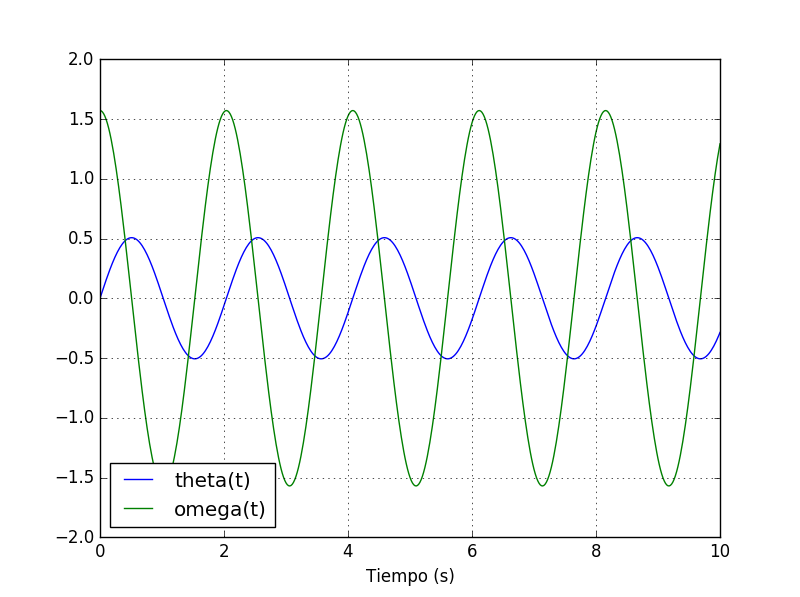
\includegraphics[width=15cm,height=9cm]{Caso1.png}
\caption{Longitud 1 m en la tierra con $\theta_=0$, $\omega_o=\pi/2$ y $b = 0$}
\end{figure}
\begin{figure}[H]
\centering
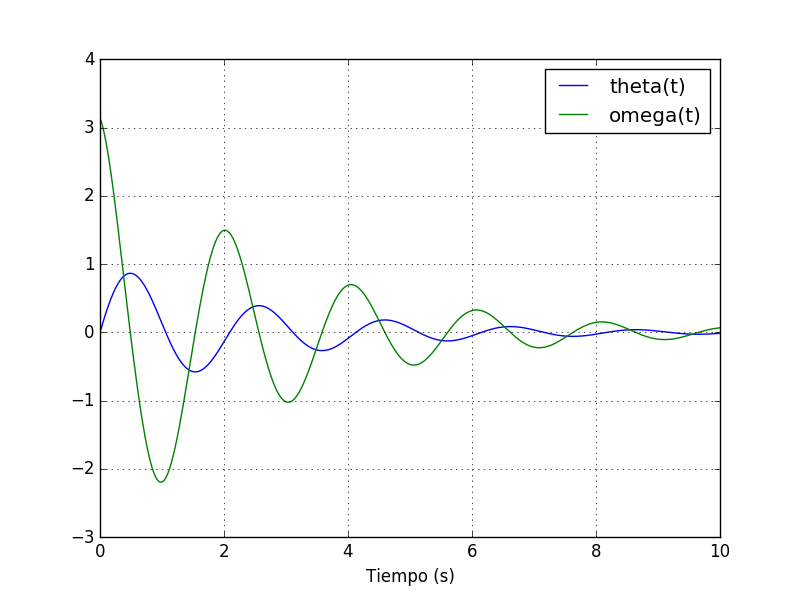
\includegraphics[width=15cm,height=9cm]{Caso2.png}
\caption{Longitud 1 m en la tierra con $\theta_=0$, $\omega_o=\pi$ y $b = 0.75$}
\end{figure}
\begin{figure}[H]
\centering
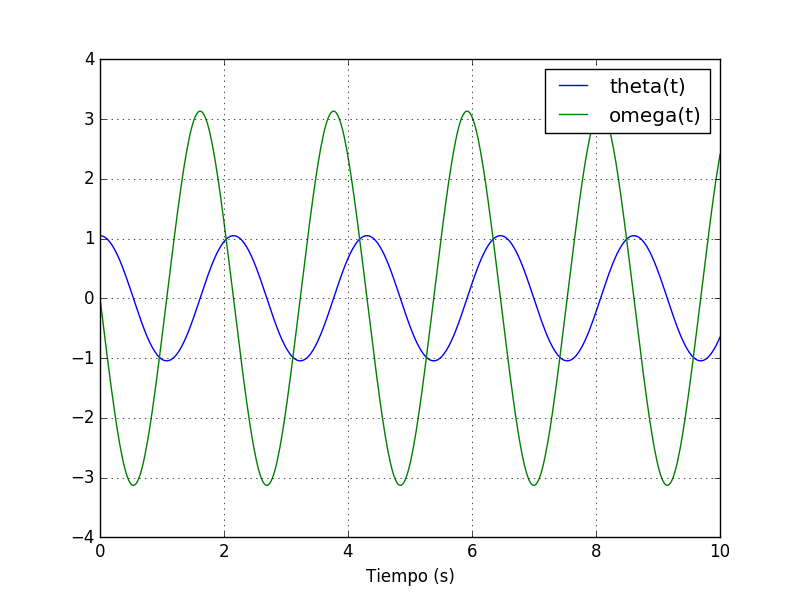
\includegraphics[width=15cm,height=9cm]{Caso3.png}
\caption{Longitud 1 m en la tierra con $\theta_=\pi/3$, $\omega_o=0$ y $b = 0$}
\end{figure}
\begin{figure}[H]
\centering
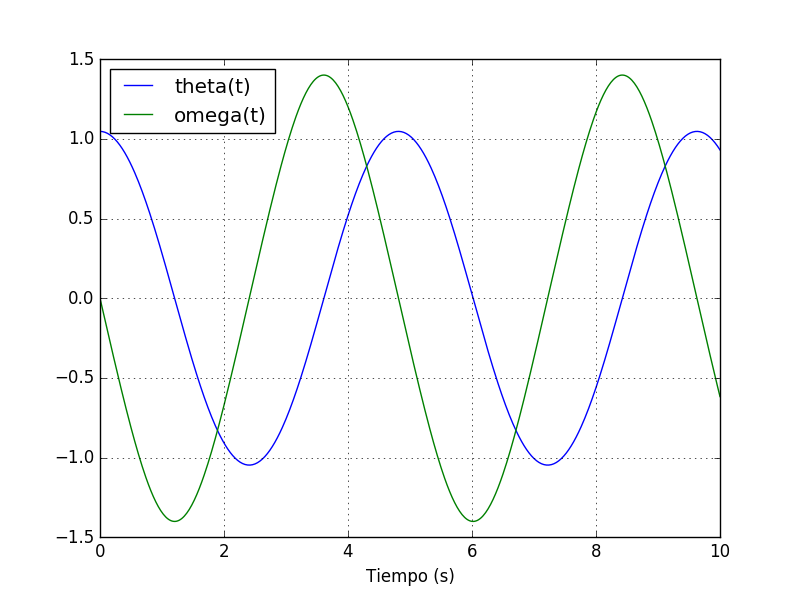
\includegraphics[width=15cm,height=9cm]{Caso4.png}
\caption{Longitud 5 m en la tierra con $\theta_=\pi/3$, $\omega_o=0$ y $b = 0$}
\end{figure}
Los resultados obtenidos son coherentes con las condiciones iniciales.
%============================================================================================================
\pagebreak

\begin{thebibliography}{3}

	\bibitem{PendWiki}
	Wikipedia,(2016)
	\emph{Pendulum (mathematics)}. Recuperado de\\
	https://en.wikipedia.org/wiki/Pendulum\_\%28mathematics\%29

	\bibitem{scipy}
	Scipy.org (2016)
	\emph{Integration and ODEs}. Recuperado de\\
	http://docs.scipy.org/doc/scipy/reference/generated/scipy.integrate.odeint.html\\\#scipy.integrate.odeint

	\bibitem{act}
	Lizárraga, C. (2016)
	\emph{Actividad 5 (2016-1)}. Recuperado de\\ 
	http://computacional1.pbworks.com/w/page/105233358/Actividad\%205\%20\\(2016-1)
	
\end{thebibliography}

\end{document}